% article example for classicthesis.sty
\documentclass[10pt,a4paper]{article} % KOMA-Script article scrartcl
\usepackage{import}
\usepackage{xifthen}
\usepackage{pdfpages}
\usepackage{transparent}
\newcommand{\incfig}[1]{%
    \def\svgwidth{\columnwidth}
    \import{./figures/}{#1.pdf_tex}
}
\usepackage{lipsum}     %lorem ipsum text
\usepackage{titlesec}   %Section settings
\usepackage{titling}    %Title settings
\usepackage[margin=10em]{geometry}  %Adjusting margins
\usepackage{setspace}
\usepackage{listings}
\usepackage{amsmath}    %Display equations options
\usepackage{amssymb}    %More symbols
\usepackage{xcolor}     %Color settings
\usepackage{pagecolor}
\usepackage{mdframed}
\usepackage[spanish]{babel}
\usepackage[utf8]{inputenc}
\usepackage{longtable}
\usepackage{multicol}
\usepackage{graphicx}
\graphicspath{ {./Images/} }
\setlength{\columnsep}{1cm}

% ====| color de la pagina y del fondo |==== %



\begin{document}
    %========================{TITLE}====================%
    \title{{  14th Lab for Forensics  }}
    \author{{Rodrigo Castillo}}
    \date{\today}

    \maketitle


    %=======================NOTES GOES HERE===================%
    \section{Rules in Yara...}
    \textbf{rule:}i starting by creating the rule for yara, i created this rule
    because i found this string in my mp3 player...
    \begin{figure}[h!]
        \centering
        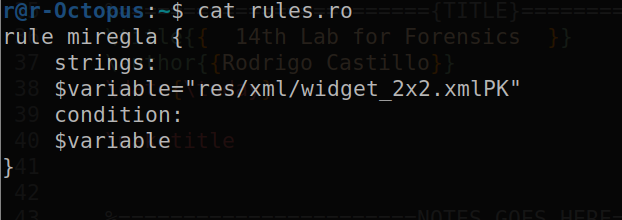
\includegraphics[width=0.8\linewidth]{rule.png}
        \caption{My Rule}
        \label{r}
    \end{figure}
    then , i proceed to check the rule in my mp3 player, so the result was
    this...
    \begin{figure}[h!]
        \centering
        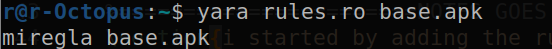
\includegraphics[width=0.8\linewidth]{detected.png}
        \caption{Rule detected on my mp3 player}
        \label{rule}
    \end{figure}
    \newpage
    \section{malicious apk search}
        i started by adding the filters $detected:true$ and $analyzed:true$ to search for android malware with :
        \begin{enumerate}
            \item {ilegal microtransactions}
            \item {priviledge for spying the victim }
            \item {priviledge for taking ilegal photos}
        \end{enumerate}
        \begin{figure}[h!]
            \centering
            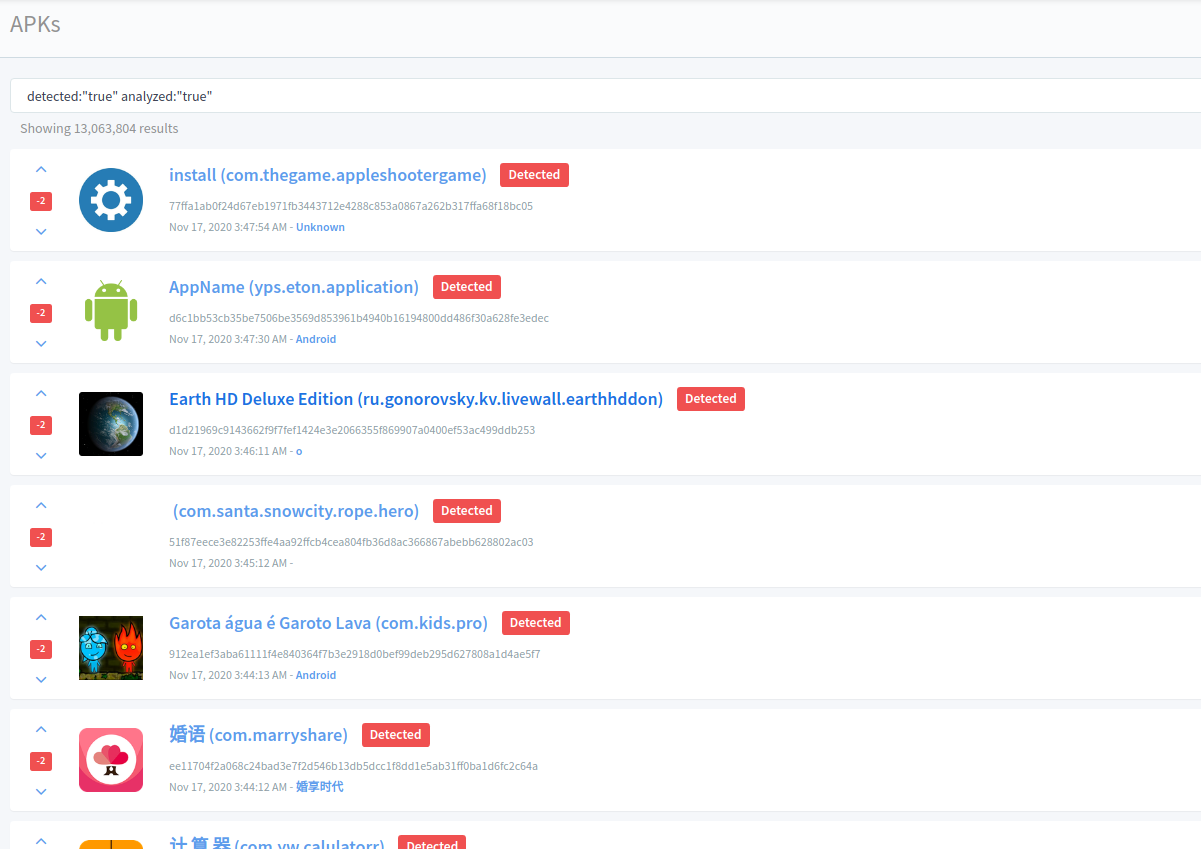
\includegraphics[width=0.8\linewidth]{apks.png}
            \caption{search}
            \label{search}
        \end{figure}
        and what i found was....
        \\
        \textbf{1:application making illegal microtransactions via sms:}
        \\
        in \textbf{videox}  we can see that is a reported application
        \begin{figure}[h!]
            \centering
            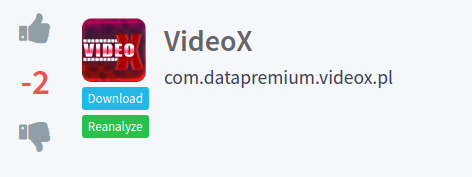
\includegraphics[width=0.8\linewidth]{videox.png}
            \caption{videox}
            \label{videox}
        \end{figure}
        if we search for the analyst reports, we can see that the application
        has 20 permissions that is a lot, also, those permissions are related
        to sms control
        \begin{figure}[h!]
            \centering
            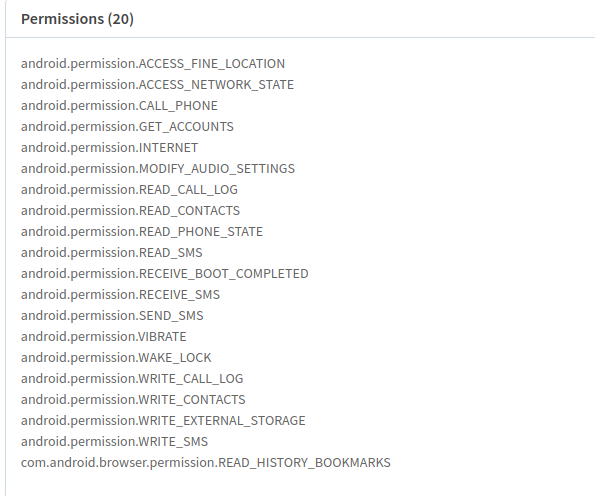
\includegraphics[width=0.8\linewidth]{videoxper.png}
            \caption{permissions of videox}
            \label{pervidx}
        \end{figure}
        then, if we check for the sms functions, we can see that its calling an sms function
        \begin{figure}[h!]
            \centering
            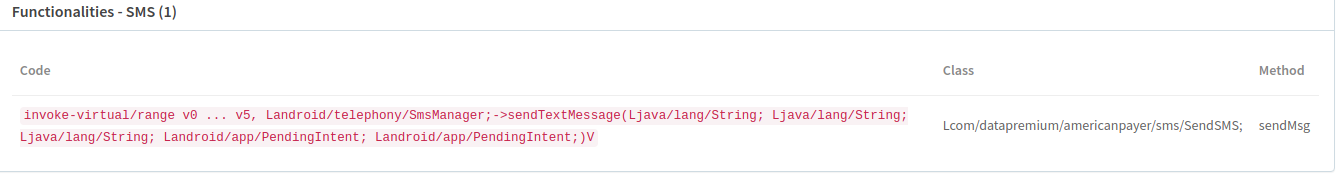
\includegraphics[width=0.8\linewidth]{sms.png}
            \caption{sms}
            \label{sms}
        \end{figure}
        this is a piece of malware that also takes advantages of other
        functionalities like phonecalls, but for the purpose of the lab i'm
        done.


        \newpage
        \textbf{application for spying...}
        this application is a piece of malware that has priviledges for spying the people who run it...
        \begin{figure}[h!]
            \centering
            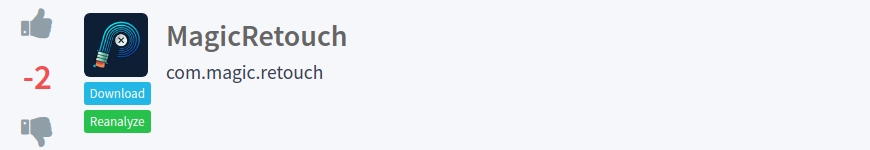
\includegraphics[width=0.8\linewidth]{spy.png}
            \caption{malware for spying}
            \label{spy}
        \end{figure}
        we can notice that if we check the file permissions that it requests...
        \begin{figure}[h!]
            \centering
            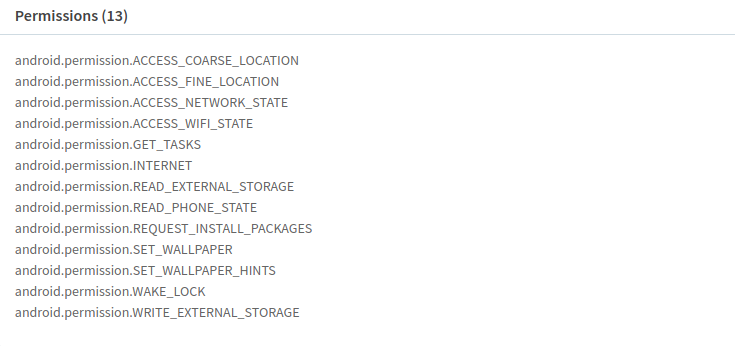
\includegraphics[width=0.8\linewidth]{spyper.png}
            \caption{spy application permissions}
            \label{fig}
        \end{figure}
        \newpage
        \textbf{application taking photos:}
        i found this application that has the priviledge of taking photos with
        the camera of the cellphone.
        \begin{figure}[h!]
            \centering
            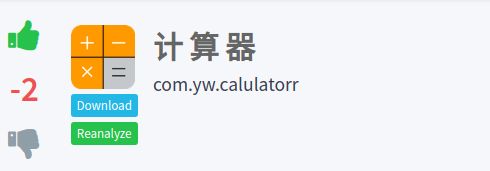
\includegraphics[width=0.8\linewidth]{photos.png}
            \caption{application that takes photos}
            \label{fotos}
        \end{figure}
        if we check for the permissions, it requiere priviledges for spying the
        victim...
        \begin{figure}[h!]
            \centering
            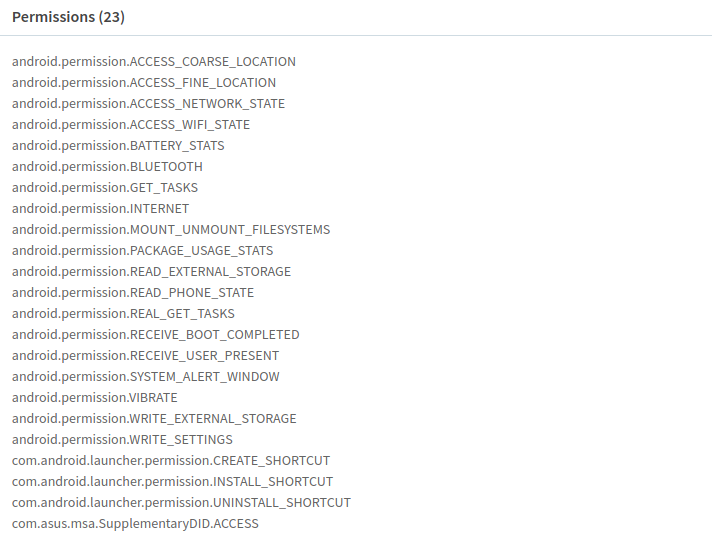
\includegraphics[width=0.8\linewidth]{SPY.png}
            \caption{priviledges for spying}
            \label{jajajaj}
        \end{figure}
        however, if we check for the function that the application its calling
        it is calling for cammera functions and its also taking both cammeras
        \begin{figure}[h!]
            \centering
            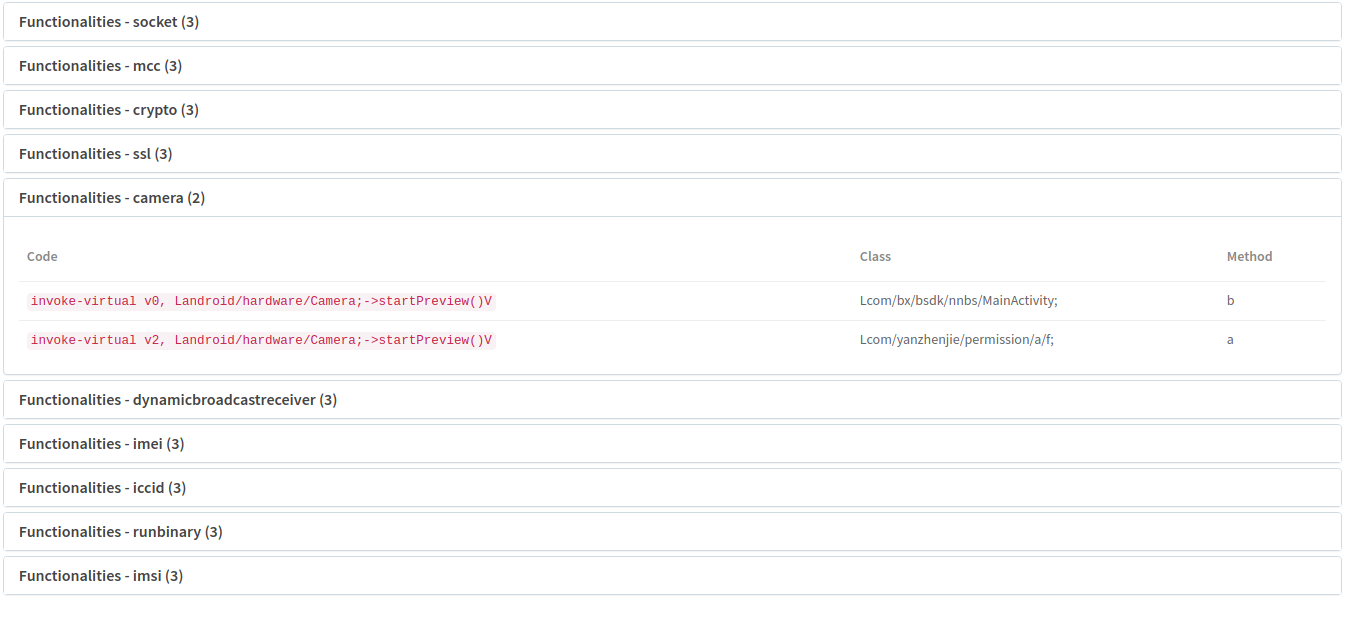
\includegraphics[width=0.8\linewidth]{camera.png}
            \caption{cammera control}
            \label{cam}
        \end{figure}
        so its a piece of malware that is spying via camera























    %=======================NOTES ENDS HERE===================%

    % bib stuff
    \nocite{*}
    \addtocontents{toc}{{}}
    \addcontentsline{toc}{section}{\refname}
    \bibliographystyle{plain}
    \bibliography{../Bibliography}
\end{document}
